\فصل{روش $Ziggurate$}

الگوریتم زیگورات:
در روش زیگورات تلاش است تا یک مصالحه بین زمان و حافظه ایجاد کند. این روش به برنامه‌نویس این امکان را می‌دهد که خود انتخاب کند چه میزان از حافظه خود را صرف ذخیره‌سازی اعداد از پیش محاسبه‌شده بکند. 
در الگوریتم زیگورات از مستطیل‌های از پیش محاسبه شده استفاده میشود که دارای "اندازه" یکسان برای پرکردن فضای زیر تابع چگالی احتمال $(PDF)$، می باشد. زیادکردن تعداد مستطیل‌ها سرعت را افزایش می‌دهد و از سویی استفاده از حافظه را بیشتر می‌کند. بنابراین کنترل مصالحه به عهده کاربر این الگوریتم است . به طور مثال در دستگاه‌هایی مانند کارت‌های هوشمند و میکروکنترلرها که حافظه محدودی دارند ، باید به سرعت کمتری تن داد در حالی که در دستگاه‌هایی که حافظه بیشتری دارند می توان از سرعت‌های بالاتری برخوردار بود. الگوریتم زیگورات برای توزیع پیوسته طراحی شده است اما می توان با درنظر گرفتن نکاتی از آن برای توزیع‌های گسسته استفاده کرد. واژه "اندازه" برای یک مستطیل  باید از مفهوم "مساحت" به مفهوم عمده " احتمال قرار گرفتن نقاط نمونه درون مستطیل " تغییر پیدا کند. 
الگوریتم زیگورات از رده الگوریتم‌های نمونه برداری ردی است و توسط $Marsaglia$  و $Tsang$  برای نمونه برداری پیوسته توزیع گوسی معرفی شد . 
  
در این الگوریتم ما می خواهیم از توزیع گوسی که میانه آن صفر و دامنه ی مورد بحث $B :=[-t_{\sigma}, t_{\sigma}]\cap \mathbb{Z}$   است استفاده کنیم.دامنه$t$ به اندازه کافی  برای  استفاده در رمزنگاری مشبکه مبنا بزرگ انتخاب می‌شود. در این‌جا توزیع پیرامون نقطه صفر است ،اما می توان یک عدد ثابت را به نمونه‌ها اضافه کرد و به این صورت می توان آن‌ها را پیرامون هر عدد غیر صفر داشت .
می توان از قسمت مثبت نمونه برداری کرد و همین نمونه‌برداری را برای قسمت منفی متناظر کرد. اگر عدد برگردانده‌شده از الگوریتم $x = 0$ باشد ، این عدد را با احتمال $\frac{1}{2}$ قبول می کنیم در غیر این صورت از میان $s\in \lbrace -1, 1\rbrace $ یک عدد انتخاب می‌کنیم و عدد نهایی که برگردانده‌می‌شود $sx$ می باشد.
\section{نمونه برداری در فضای مثبت }

در این روش از تابع چگالی احتمال $(PDF)$ استفاده می‌شود.  تابع $(PDF)$ را به یک فضا به نام $A$  که شامل $m$ مستطیل افقی است که مساحت‌های برابری دارند  ، تبدیل می‌کنیم همان‌طور که در شکل ... نشان داده‌شده‌است.

    \begin{figure}[!htb]
      	\minipage{1\textwidth}
      	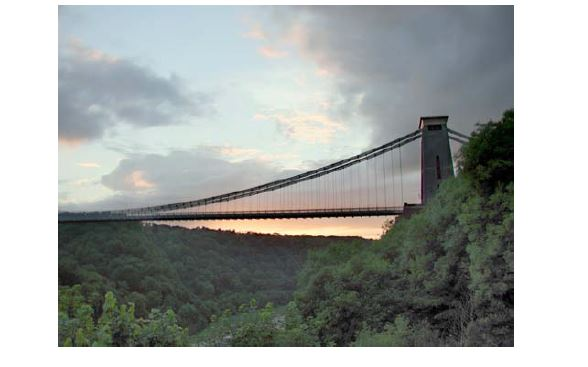
\includegraphics[width=\linewidth]{images/retinex1}
      	\caption{retinex}\label{fig:logtonemap}
      	\endminipage\hfill
      	% 	\centerline{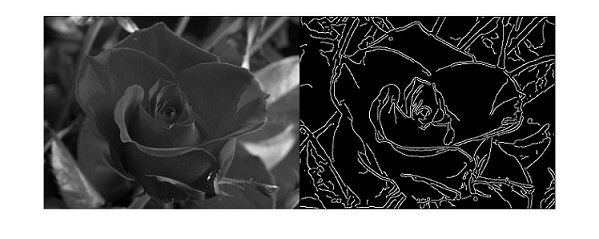
\includegraphics{images/cannyexample2}}
      \end{figure}

یک جفت عدد $(x_{i},y{i})$ که نشان‌دهنده گوشه پایین مستطیل $R_{i}$ است ،$1\< i \< m - 1$ ، را نگه می داریم. 
هر مستطیل را می توان به دو مستطیل  سمت راست$ R^{r}_{i}$ و  سمت چپ$ R^{l}_{i}$ تقسیم کرد . مستطیل سمت چپ به طور کامل زیر نمودار $PDF$گوسی قرار دارد و مستطیل سمت راست تا حدودی زیر نمودار $PDF$  قرار دارد. می‌توان برای نمونه به $R_{6}$  در شکل ... نگاه کرد.
برای این‌که بتوان نمونه $x \leq t_{\sigma}$  در $\mathbb{R}^{+}_{0}$  انتخاب کرد ، یک مستطیل به صورت تصادفی انتخاب کنیم ، ابتدا یک عدد به صورت یکنواخت از بین 1 تا m  انتخاب می کنیم. سپس یک x به صورت یکنواخت بین 0 تا x_{i} انتخاب می کنیم  و آن را x’  می نامیم. اگر x’ <=  x_{i – 1}   یا x’  درون R^{l}_{i} قرار دارد . بنابراین این عدد مورد پذیرش ما هست ، در غیر این صورت x’  در R^{r}_{i} واقع شده است. در این شرایط ما از نمونه برداری ردی استفاده می کنیم . یک نمونه همانند \gama  در بازه  [y_{i+1}, y_{i}] به صورت یکنواخت انتخاب می کنیم . سپس اگر \gama + y_{i+1} <= \row_{\sigma}(x’) یک عدد از زیر نمودار انتخاب کرده‌ایم ، عدد را می پذیریم و x’  را برمی گردانیم. در غیر این صورت نمونه را رد می کنیم و دوباره تمام مراحل را تکرار می کنیم.
این الگوریتم در واقع همان الگوریتم نمونه برداری ردی است که قسمت اول الگوریتم (نمونه برداری یک نقطه در فضای زیر نمودار) بهتر شده است . در این روش تمام مستطیل ها سایز برابر دارند بنابراین اختمال آنکه نقطه انتخاب شده در مستطیل ها باشد برابر است. بنابراین می توان ابتدا از بین مستطیل‌ها نمونه برداری کرد و سپس یک نقطه از بین مستطیل‌ها انتخاب کرد.
بیشترین هزینه این الگوریتم‌ در محاسبه ρσ(x0)  است . اگر x’ در مستطیل R^{l}_{i} واقع نشده باشد باید ρσ(x0)   را محاسبه کرد.  اگر این نمونه رد شود هزینه بیشتری دارد. بنابراین زیگورات یک مصالحه بین زمان و حافظه است که به وسیله تعداد مستطیل‌ها کنترل می شود. اگر تعداد بیشتری مستطیل استفاده کنیم ، نسبت بین مستطیل  چپ و راست تغییر می کند به طوری که مستطیل چپ نسبت به مستطیل راست ، بزرگتر می شود. بنابراین با احتمال بیشتری می‌توان  یک x’  را بدون محاسبه ρσ(x0)   پذیرفت.  همچنین در صورتی که تعداد مستطیل‌ها زیادتر شود فضای A  به فضای زیر PDF نزدیک‌تر است . در نتیجه A/C  که موجب رد شدن نمونه می شود ، کاهش می یابد. اما برای هر مستطیل اضافی باید نقاط مرتبط با این مستطیل نگه‌داری شود بنابراین به استفاده بیشتر از حافظه نیاز دارد.
برای گسسته!
مقایسه با بقیه روشها! (510)

      \begin{figure}[!htb]
      	\minipage{1\textwidth}
      	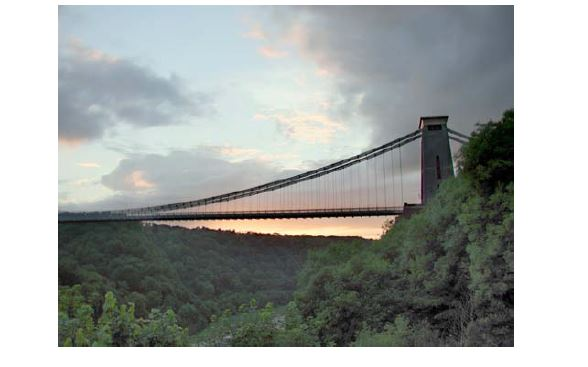
\includegraphics[width=\linewidth]{images/retinex1}
      	\caption{retinex}\label{fig:logtonemap}
      	\endminipage\hfill
      	% 	\centerline{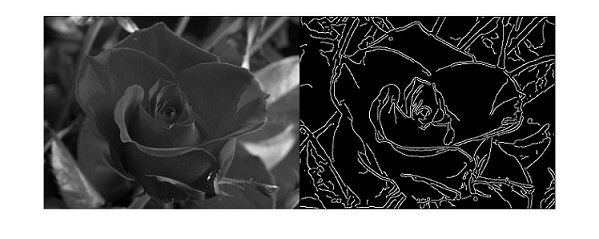
\includegraphics{images/cannyexample2}}
      \end{figure}

  
